

\setcounter{section}{0}
%==========================================

%\section*{第一章:相对论重离子碰撞}


\setcounter{figure}{0}
\setcounter{table}{0}
\setcounter{equation}{0}




\chapter{RHIC-STAR实验装置} \vskip -0.5cm
% To add a non numbered chapter
%\addcontentsline{toc}{第一章}{相对论重离子碰撞}
% To insert this section on the table of contents

\begin{figure}[htbp]
\centering
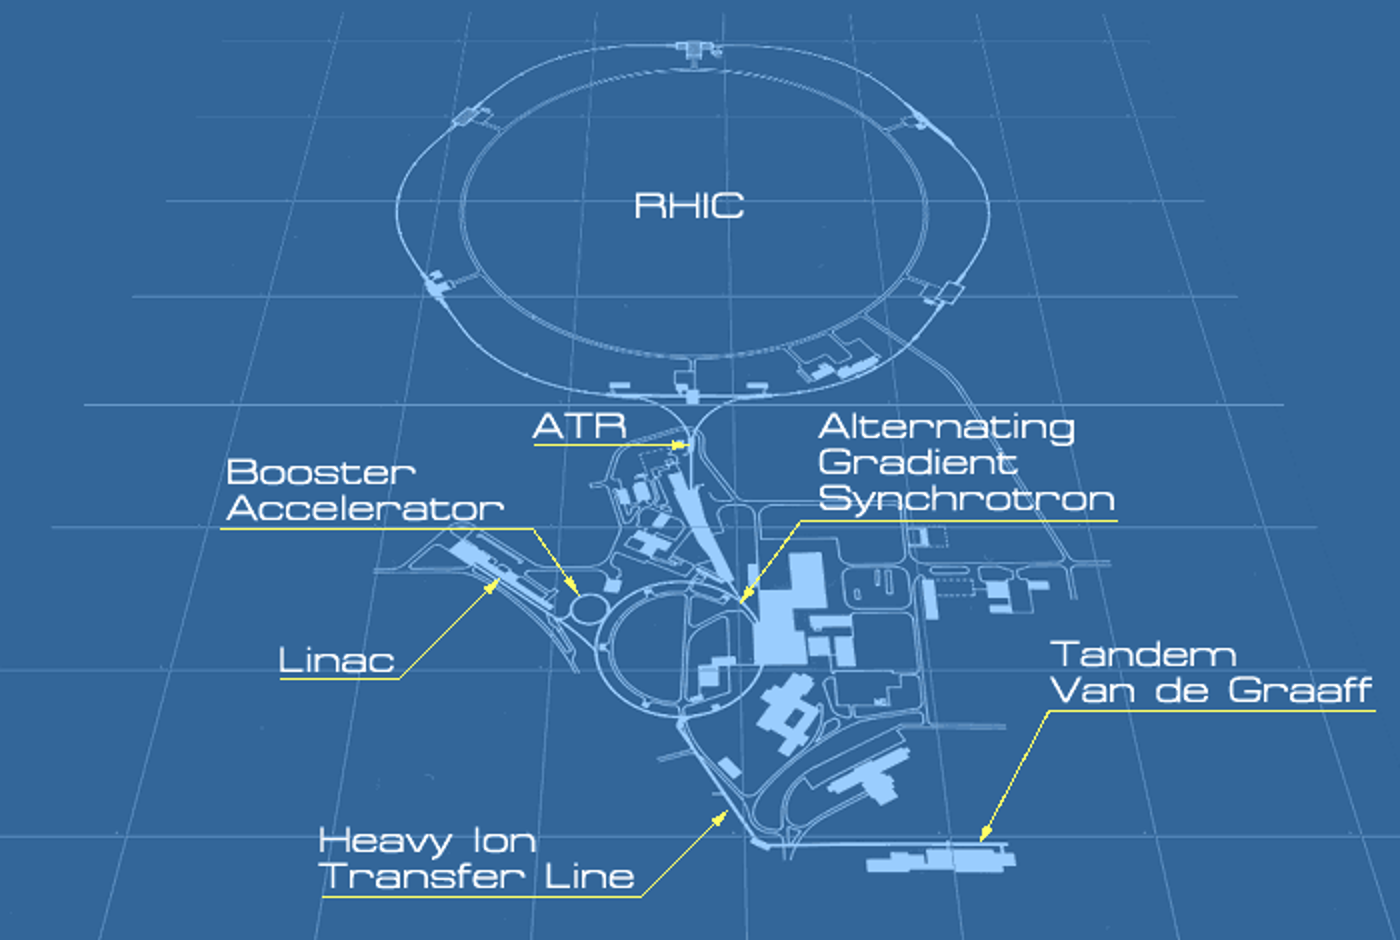
\includegraphics[width=0.8\textwidth]{./figures/RHIC.png}
\caption{位于BNL的相对论重离子对撞机RHIC的加速器示意图。}
\label{Fig:RHIC}
\end{figure}


%\renewcommand{\thechapter}{\arabic{chapter}} % change the chapter counter to be 1
%\thispagestyle{fancy}
位于美国布鲁克海文国家实验室(Brookhaven National Laboratory,简称:BNL)的相对论重离子对撞机(The Relativistic Heavy-Ion Collider, 简称:RHIC)\cite{harrison2003rhic}是世界上第一个专用的重离子对撞机,建立与2000年,从2001年开始为科学家提供了满能量的电子束流~\cite{qgp}。
RHIC是世界上第一个运行的重离子对撞机\cite{harrison2003rhic}。

图\ref{Fig:RHIC}是它的结构示意图。在RHIC装置上,重离子被注入对撞机之前是通过范德格拉夫串列静电加速器(Tandem Van De Graaff),增强器(The Booster Synchrotron),交变梯度同步加速器(Alternating Gradient Synchrotron, 简称:AGS)预加速的~\cite{qgp,harrison2003rhic}。
为了加速一束金原子核,我们先通过脉冲溅射离子源得到带负电的金离子,然后利用第一级的范德格拉夫串列静电加速器进行加速;在这里部分核外电子被位于内部高压终端的箔片剥离;随后带正电的金离子通过第二级装置加速到每核子1. MeV~\cite{harrison2003rhic, qgp}。这些带正电的离子通过传输线到达带有射频电场的增强器中~\cite{qgp}。在增强器中金离子被分为三束团并加速到每核子78MeV,增强器出口的箔片会把所有核外电子剥离,从而我们得到了干净的金原子核,然后金原子核将被注入到AGS之中,AGS会把三束金离子加速到10.8 GeV并注入RHIC环中~\cite{qgp,harrison2003rhic}。RHIC环有两个,分别被称为“蓝(Blue)”环(顺时针方向)和"黄(Yellow)"环(逆时针方向),它们的周长为3.834$Km$,离子在两条环中具有相反的运动方向~\cite{qgp,harrison2003rhic}。RHIC环的束流是建设在同一个水平面上的两个非圆形同心超导磁铁环,两个环在六个不同的位置相互交叉~\cite{qgp,harrison2003rhic},也就是说RHIC环上有6个对撞点,但其中只有4个对撞点装上了探测器,分别为BRAHMS(在2点钟方向);STAR(6点钟方向);PHENIX(8点钟方向);以及PHOBOS(10点钟方向)。目前只有STAR实验装置还在运行中,PHENIX正在升级中。

至今RHIC上进行了一系列的不同碰撞系统、碰撞的能量,其中包括p+p, p+Al, p+Au, d+Au, $\mathrm{He^3}$+Au, Cu+Cu, Cu+Au, Au+Au, U+U, Ru+Ru, Zr+Zr对撞,以及一些低能的固定靶实验(Au+Au)。

\bigskip

\section{STAR探测器}

RHIC上的螺线管径迹探测器(The Solenoidal Tracker At RHIC,简称:STAR)主要是用于研究了解重离子碰撞的时空演化过程,以及碰撞产生的“小爆炸“中所产生的QGP的性质。STAR探测器是由很多的子探测器组成\cite{ackermann2003star}。%主要包括磁铁\cite{bergsma2003star},磁铁是为了提供沿圆筒轴向方向上的均匀磁场;
\begin{figure}[htbp]
\centering
\includegraphics[width=\textwidth,clip]{figure/STAR_detector.png}
\caption{STAR探测器示意图。}
\label{fig:star_overview}
\end{figure}
 每个子探测器都有其特定功能,例如TPC可用于跟踪,在较低的横向动量范围内测量带电粒子的动量,TOF可以识别在较高的横向动量范围内的带电粒子以及VPD可以测量初级碰撞顶点的位置, 适用于重离子碰撞中的逐事件特征。
 图\ref {fig:star_overview}是STAR检测器的示意图。零度量能器(Zero Degree Calorimeters,简称:ZDC)\cite{adler2001rhic}主要是用于探测未参与碰撞的重子的位置信息,可用于重建一阶事件平面;束流计数器(Beam Beam Counters,简称:BBC)\cite{whitten2008beam}主要用统计前向快度区的粒子数,可以通过它的反应作为事件触发的条件和束流质量的检测。时间投影室(Time Projection Chamber,简称:TPC)\cite{anderson2003star},它是STAR的主要的径迹探测器,它提供了带电粒子的碰撞点,用以重建带电粒子的运动径迹,并通过测量电子在磁场中的曲率从而得到粒子的动量并通过电离能损来鉴别粒子,关于TPC的具体功能将在下面进行展开介绍;飞行时间探测器(Time of Flight, 简称:TOF)\cite{bonner2003single,llope2004tofp,llope2005large},它用于测量带电粒子从碰撞顶点飞到探测器的时间,然后加上TPC中提供的信息从而可以计算粒子的静止质量,即可以用于做粒子鉴别,且其效果非常好;
顶点位置探测器(upgraded Pseudo Vertex Position Detectors 简称:upVPD)\cite{llope2014star},它位于束流方向距离对撞点约5.7m的两端,主要是测量束流方向对撞点的位置信息,可以为TOF提供对撞点的起始时间,还可以通过碰撞点的位置对碰撞事件进行初步筛选。
以下将对本文分析中所用到的主要探测器进行介绍。




\subsection{时间投影室}

\begin{figure}[htbp]
\centering
\includegraphics[width=0.8\textwidth]{./figure/STAR_TPC.png}
\caption[TPC探测器 ]{STAR TPC探测器示意图 \cite{anderson2003star}}
\label{Fig:STAR_TPC}
\end{figure}
时间投影室(Time Projection Chamber,简称TPC)~\cite{anderson2003star}是STAR最主要的径迹探测器,主要用来记录带电粒子的运动轨迹及其动量。
TPC综合来电场、磁场并且包含了敏感气体的粒子探测器,它可以提供粒子的三维坐标信息。
通过TPC提供的带电粒子运动轨迹的信息,可以重建事件的碰撞顶点、测量离子的横动量信息,而且可以通过电离能量损失(ionization energy loss,\dEdx)对带电粒子进行鉴别。
 图.\ref{Fig:STAR_TPC}给出的是TPC探测器的示意图。它的赝快度(pseudo-rapidity, 通常用$\eta$表示)接收范围为 $-1 < \eta <1$,而且它具有全方位角的接受度($0<\phi<2\pi$)。TPC主要由两部分组成,一部分是气体漂移室(Drift Chamber),另外一部分是多丝正比室(Multi-Wire Proportional Chamber,简称:MWPC)。如图~\ref{Fig:STAR_TPC2}所示气体漂移室是与束流同轴的圆筒,在圆筒两侧是多丝正比室。
TPC的长度为4.2m,内径为0.5m,外径为2m。当外部磁场提供的磁场强度为0.5T时,TPC所能测量的动量范围为是$0.10 <p_{T}<30$~GeV/c。

\begin{figure}[htbp]
\centering
\includegraphics[width=0.8\textwidth]{./figure/STAR_TPC2.png}
\caption{TPC读出扇形示意图 \cite{anderson2003star}}
\label{Fig:STAR_TPC2}
\end{figure}


在STAR实验中,对撞产生了大量的带电粒子,TPC处在均匀磁场之中因此这些带电粒子的运动轨迹为螺旋形,且该螺旋形在$x-y$平面内的投影是一个圆圈。STAR的读出系统是基于多丝正比室\cite{anderson2003star},TPC的两端分别有12个扇形,如图如图~\ref{Fig:STAR_TPC2}所示每个扇区分为内层和外层。外层扇区有32行读出片,读出片的面积为6.2mm $\times$ 19.5mm,总计3942个,内层扇区有13行读出片,读出片的面积为2.85mm $\times$ 11.5mm, 总计1750 个。外层读出片面积较大,间距较小,能够提供好的粒子能损测量。内层读出片面积小,间距大,位置分辨率较高。每个读出片的位置是固定的,所以它能提供X 和Y 的坐标信息。在Z轴方向,将电子从中心膜到多丝正比室漂移事件分为512个时间段,每个约为100ns。多丝正比室的读出系统能够满足相对论重离子碰撞高频率高粒子数产生的事件采集,金金碰撞中,其读出频率为2KHz。
当带电粒子在漂移室中运动时,每隔一段距离就会与气室中的气体发生相互作用而电离出电子,粒子的漂移速度在130V/cm的均匀电场下的速度约为5.45cm/$\mu$s ,漂移的电子被在TPC的两端的读出系统收集后转换成电信号,然后传送到STAR的数据采集系统,因为读出板只有45层(在后期升级中总共有55层,目前分析的数据都是45层),因此在TPC探测器中运动的粒子在读出板上最多有45 个击中点(即nHitMax最大为45),也就是总共最多可以提供45个位置信息用来拟合带电粒子的径迹。在后期的数据重建的过程中,利用卡尔曼滤波的方法对TPC所采集的碰撞信息对带电粒子径迹进行拟合、计算该径迹的电离能量损失(\dEdx )。
粒子的平均电离能损($\langle dE/dx \rangle$) 由Bethe-Bloch经验公式给出:
\begin{equation}
\label{eq:bethe_bloch}
-\frac{dE}{dX} = 4\pi N_{A}r_{e}^{2}m_{e}c^{2}z^{2}\frac{Z}{A}\frac{1}{\beta^{2}}\big[\frac{1}{2}ln\frac{2m_{e}c^{2}\beta^{2}\gamma^{2}}{I^{2}} - \beta^{2} - \frac{\delta}{2} \big]
\end{equation}
其中,$N_{A}$是阿伏加德罗常数,$I$是所穿越物质的平均激发能,$z$是入射粒子的电荷量,$A$是核子数,$m_{e}$是电子质量,$r_{e}$是电子的经典半径,$\delta$为密度效应修正参数,$\beta$为粒子的速度,$Z$是所穿越物质的原子序数,$\beta = v/c$,$\gamma = 1/\sqrt{1-\beta^{2}}$。
\begin{figure}[htbp]
\centering
\includegraphics[width=0.8\textwidth,clip]{figure/dEdx_39GeV.png}
\caption{带电粒子的电离能损分布图}
\label{fig:tpc_dedx}
\end{figure}
实验中我们通过将粒子的电离能损与该粒子的理论值做比较,以得到他们的标准偏差$n\sigma$,以此来衡量该粒子是否为某个粒子的一个标准:
\begin{equation}
n\sigma = \frac{1}{R} \frac{\langle dE/dx|_{measure} \rangle}{\langle dE/dx|_{theory} \rangle}
\label{eq:nsigma}
\end{equation}
式中的$R$是电离能损分辨率。$n\sigma$越小则证明该粒子的确定性越高。图~\ref{fig:tpc_dedx}是TPC中带电粒子的电离能损随动量的分布图,图中的虚线表示不同粒子的理论计算值随动量的关系。在一定程度上TPC探测器有良好的粒子的鉴别功能,在一些区域则没有表现处很好的鉴别能力,特别是在动量比较大的时候。这就需要加上TOF的信息以提高粒子鉴别的准确度。


\subsection{飞行时间探测器}

\begin{figure}[htbp]
\centering
\includegraphics[width=0.67\textwidth,clip]{figure/STAR_TOF_tray.png}
\caption{STAR飞行时间探测器上的多气隙电阻板室的结构示意图\cite{llope2005large}}
\label{fig:tof_mrpc_view}
\end{figure}

STAR飞行时间探测器(Time of Filght,简称TOF)\cite{llope2005large},它主要用来测量粒子的飞行时间,提高STAR探测器的粒子鉴别能力。它位于TPC的外侧,由120个条形板组成\cite{llope2005large}(TPC的东西两侧各60个)。每个条形板包含34个沿束流方向放置的多气隙电阻板室(Multi-gap Resistive Plate Chamber ,简称:MRPC) 模块\cite{llope2005large}。其赝快度覆盖范围是$|\eta|<1$,方位角是全空间接收的($2\pi$)。
每个TOF的条形板由32个MRPC模块组成。图.\ref{fig:tof_mrpc_view}给出的是STAR飞行时间探测器上的多气隙电阻板室的结构示意图。
MRPC由上下两层读出电极和中间的多层平行玻璃电阻板组成\cite{llope2005large}。玻璃与玻璃之间由尼龙丝隔开,形成均匀的6个气隙。外层玻璃板通过石墨电极加入高压,这样每个气隙之间就充满来均匀的强电场。当带电粒子穿过MRPC时,在气隙中电离的电子会立刻引起雪崩。因为玻璃板是半绝缘的,因此不会对信号造成干扰,那么读出电极上的感应信号就是各个气隙中雪崩的总和。
因为TOF与碰撞顶点的距离$L$是已知的,因此带电粒子的速度($\beta$)和质量($m$)为:
\begin{align}
\beta &= \frac{v}{c}=\frac{L}{c\Delta t}\\
m^{2}&=p^{2}(\frac{1}{\beta}-1)
\end{align}
这里的 $\beta = p/E $ ,$E = \sqrt{p^{2} + m^{2}}$,  $p$是粒子在TPC所测量的动量,$\Delta t$ 是TOF测量的开始时间和VPD测量的停止时间的差值。
\begin{figure}[htbp]
\centering
\includegraphics[width=0.6\textwidth,clip]{figure/mass2_39GeV.png}
\caption{STAR-TOF测量的粒子质量与动量的关系}
\label{fig:tof_beta}
\end{figure}

图.\ref{fig:tof_beta}是在 {\sNN} = 39 GeV下测量的粒子质量与动量的关系。从图中可以清楚的看到不同粒子所属不同颜色的带子是相互分离的,即利用TOF和TPC所提供的信息能够很好的把粒子鉴别清楚。强大的粒子鉴别能力无疑为我们研究QGP的演化过程和性质提供了强大的武器。



\subsection{重味探测器(Heavy Flavor Tracker)}
2014-2016年在RHIC运行的数据采集期间,STAR实验中加入重味探测器(Heavy Flavor Tracker,简称:HFT)。如图~\ref{fig:hftPixel}所示,可以看到它是由三个硅子探测器组成,包括在最外面的一层条形硅探测器(Silicon Strip Detector,简称SSD )~\cite{ARNOLD2003652};在中间一层的硅径迹探测器( Intermediate Silicon Tracker,简称:IST);以及最里的两层像素探测器(PIXEL)\cite{HLTPIXEL,CONTIN201860}。在这三个子探测器的共同作用下对方位角的覆盖范围是$2\pi$。
\begin{figure}[htbp]
\centering
\includegraphics[width=0.67\textwidth,clip]{Figures_Use/HFT.png}
\caption{重味探测器概述图~\cite{Hao_2014}}
\label{fig:hftPixel}
\end{figure}
根据HFT探测器的信息,由于其出色的分辨率,在重建事件碰撞初级顶点的时候起到了很大的作用。在只有TPC和VPD的情况下,筛选好事件的一个重要标准是其重建的碰撞顶点在束流方向的距离不大于30cm。但通过HFT探测器所提供的信息,我们可以更加精确的重建事件的碰撞顶点,此时我们选的好事件的评判标准是重建的碰撞顶点在束流方向的距离不大于6cm。加入HFT的优势显而易见。在我们下面的分析中用到了run16的Au + Au 200 GeV 的数据,采集过程中安装了HFT,因此在此对其做一个简单介绍。



